\documentclass[border=4pt]{standalone}

\usepackage{amsmath}
\usepackage{tikz}
\usepackage{mathdots}
\usepackage{yhmath}
\usepackage{cancel}
\usepackage{color}
\usepackage{siunitx}
\usepackage{array}
\usepackage{multirow}
\usepackage{amssymb}
\usepackage{gensymb}
\usepackage{tabularx}
\usepackage{booktabs}
\usetikzlibrary{fadings}
\usetikzlibrary{patterns}


\begin{document}
 


\tikzset{every picture/.style={line width=0.75pt}} %set default line width to 0.75pt        

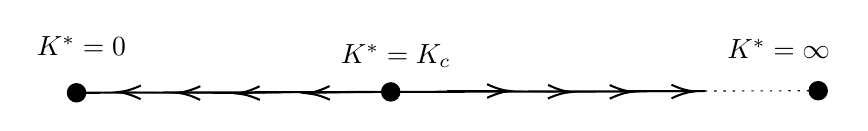
\begin{tikzpicture}[x=0.75pt,y=0.75pt,yscale=-1,xscale=1]
%uncomment if require: \path (0,300); %set diagram left start at 0, and has height of 300

%Straight Lines [id:da5525635838013163] 
\draw [line width=0.75]    (114,129.33) -- (416.75,128.5) ;


%Shape: Circle [id:dp6627305429374732] 
\draw  [fill={rgb, 255:red, 0; green, 0; blue, 0 }  ,fill opacity=1 ] (109.58,129.33) .. controls (109.58,126.89) and (111.56,124.92) .. (114,124.92) .. controls (116.44,124.92) and (118.42,126.89) .. (118.42,129.33) .. controls (118.42,131.77) and (116.44,133.75) .. (114,133.75) .. controls (111.56,133.75) and (109.58,131.77) .. (109.58,129.33) -- cycle ;
%Straight Lines [id:da6448275641896342] 
\draw    (162.67,129.33) -- (136,129.02) ;
\draw [shift={(134,129)}, rotate = 360.66999999999996] [color={rgb, 255:red, 0; green, 0; blue, 0 }  ][line width=0.75]    (10.93,-3.29) .. controls (6.95,-1.4) and (3.31,-0.3) .. (0,0) .. controls (3.31,0.3) and (6.95,1.4) .. (10.93,3.29)   ;

%Straight Lines [id:da3700498741940408] 
\draw    (322.75,128.5) -- (350.08,128.97) ;
\draw [shift={(352.08,129)}, rotate = 180.98] [color={rgb, 255:red, 0; green, 0; blue, 0 }  ][line width=0.75]    (10.93,-3.29) .. controls (6.95,-1.4) and (3.31,-0.3) .. (0,0) .. controls (3.31,0.3) and (6.95,1.4) .. (10.93,3.29)   ;

%Straight Lines [id:da987300602570016] 
\draw    (352.08,129) -- (379.83,128.84) ;
\draw [shift={(381.83,128.83)}, rotate = 539.6800000000001] [color={rgb, 255:red, 0; green, 0; blue, 0 }  ][line width=0.75]    (10.93,-3.29) .. controls (6.95,-1.4) and (3.31,-0.3) .. (0,0) .. controls (3.31,0.3) and (6.95,1.4) .. (10.93,3.29)   ;

%Straight Lines [id:da9813028156171861] 
\draw    (381.83,128.83) -- (409.58,128.68) ;
\draw [shift={(411.58,128.67)}, rotate = 539.6800000000001] [color={rgb, 255:red, 0; green, 0; blue, 0 }  ][line width=0.75]    (10.93,-3.29) .. controls (6.95,-1.4) and (3.31,-0.3) .. (0,0) .. controls (3.31,0.3) and (6.95,1.4) .. (10.93,3.29)   ;

%Shape: Circle [id:dp4883251883549766] 
\draw  [fill={rgb, 255:red, 0; green, 0; blue, 0 }  ,fill opacity=1 ] (466.92,128.33) .. controls (466.92,125.89) and (468.89,123.92) .. (471.33,123.92) .. controls (473.77,123.92) and (475.75,125.89) .. (475.75,128.33) .. controls (475.75,130.77) and (473.77,132.75) .. (471.33,132.75) .. controls (468.89,132.75) and (466.92,130.77) .. (466.92,128.33) -- cycle ;
%Straight Lines [id:da9333745775510272] 
\draw  [dash pattern={on 0.84pt off 2.51pt}]  (416.75,128.5) -- (471.33,128.33) ;


%Shape: Circle [id:dp4811776160172614] 
\draw  [fill={rgb, 255:red, 0; green, 0; blue, 0 }  ,fill opacity=1 ] (260.96,128.92) .. controls (260.96,126.48) and (262.94,124.5) .. (265.38,124.5) .. controls (267.81,124.5) and (269.79,126.48) .. (269.79,128.92) .. controls (269.79,131.36) and (267.81,133.33) .. (265.38,133.33) .. controls (262.94,133.33) and (260.96,131.36) .. (260.96,128.92) -- cycle ;
%Straight Lines [id:da512853355595918] 
\draw    (191.33,129.67) -- (164.67,129.36) ;
\draw [shift={(162.67,129.33)}, rotate = 360.66999999999996] [color={rgb, 255:red, 0; green, 0; blue, 0 }  ][line width=0.75]    (10.93,-3.29) .. controls (6.95,-1.4) and (3.31,-0.3) .. (0,0) .. controls (3.31,0.3) and (6.95,1.4) .. (10.93,3.29)   ;

%Straight Lines [id:da13782239139786423] 
\draw    (227.25,129) -- (193.33,129.63) ;
\draw [shift={(191.33,129.67)}, rotate = 358.94] [color={rgb, 255:red, 0; green, 0; blue, 0 }  ][line width=0.75]    (10.93,-3.29) .. controls (6.95,-1.4) and (3.31,-0.3) .. (0,0) .. controls (3.31,0.3) and (6.95,1.4) .. (10.93,3.29)   ;

%Straight Lines [id:da7085462315276623] 
\draw    (260.96,128.92) -- (227.04,129.55) ;
\draw [shift={(225.04,129.58)}, rotate = 358.94] [color={rgb, 255:red, 0; green, 0; blue, 0 }  ][line width=0.75]    (10.93,-3.29) .. controls (6.95,-1.4) and (3.31,-0.3) .. (0,0) .. controls (3.31,0.3) and (6.95,1.4) .. (10.93,3.29)   ;

%Straight Lines [id:da5046057046718395] 
\draw    (292.25,128.5) -- (320.75,128.5) ;
\draw [shift={(322.75,128.5)}, rotate = 180] [color={rgb, 255:red, 0; green, 0; blue, 0 }  ][line width=0.75]    (10.93,-3.29) .. controls (6.95,-1.4) and (3.31,-0.3) .. (0,0) .. controls (3.31,0.3) and (6.95,1.4) .. (10.93,3.29)   ;


% Text Node
\draw (116.33,107) node    {$K^{*} =0$};
% Text Node
\draw (452.33,108.33) node    {$K^{*} =\infty $};
% Text Node
\draw (267.83,111.5) node    {$K^{*} =K_{c}$};


\end{tikzpicture}

\end{document}
